\chapter{Results}
\label{ch:results}

This chapter reports the outputs of the Framingham case study in three parts. First, it compares the current \gls{fps} routing baseline against \gls{bra}-generated routes for currently assigned riders. Second, it tests whether expanded eligibility scenarios can be served with the available fleet. Third, it uses Pareto fronts to show how fleet use, coverage, cost, emissions, and stop use trade off under the modeled assumptions.

Current routing is shaped by the interaction between district school choice policies and Massachusetts transportation requirements. Under Massachusetts General Laws (MGL Ch. 71, Section 68), districts must provide free transportation to K-6 students living more than 2 miles from school. As shown in \autoref{fig:geospatial}, this policy is consistent with an incentive for some families in Framingham to select schools farther from home in order to secure transportation coverage. This pattern appears especially visible among lower-income and minority households in the southern part of the city, as well as among families of students with disabilities.

\begin{figure}[!htbp]
    \centering
    \begin{subfigure}{0.33\textwidth}
        \subcaption{Students in \gls{fps} by distance to school}
        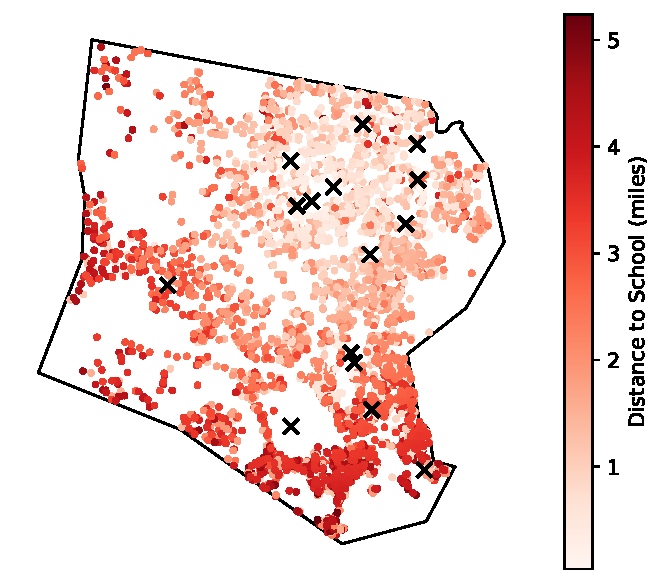
\includegraphics[width=0.99\textwidth, alt={Map of student locations in Framingham colored by distance to school. Darker red points indicate students farther from school, with schools marked by black X symbols.}]{figures/students_distance_to_school.pdf}
    \end{subfigure}
    \begin{subfigure}{0.33\textwidth}
        \subcaption{Distance to school for students with disabilities}
        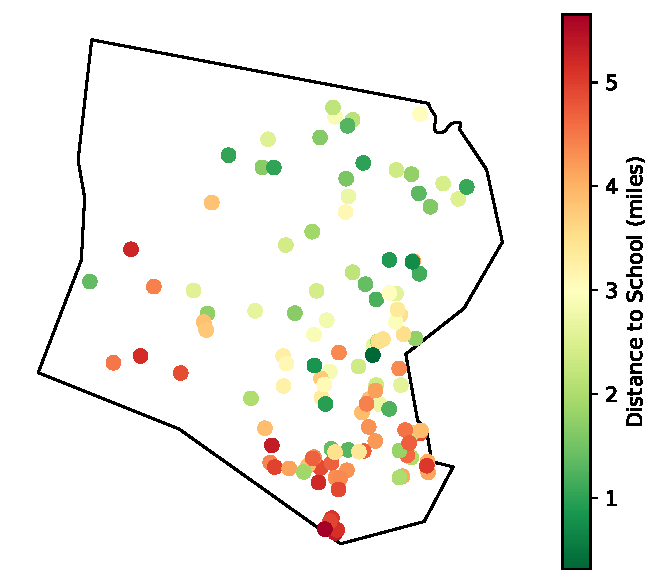
\includegraphics[width=0.99\textwidth, alt={Map of stops used by students with disabilities in Framingham colored by distance to school. Points show student locations, and warmer colors indicate longer school distances.}]{figures/special_education_students.pdf}
    \end{subfigure}
    \begin{subfigure}{0.33\textwidth}
        \subcaption{Median income by block group}
        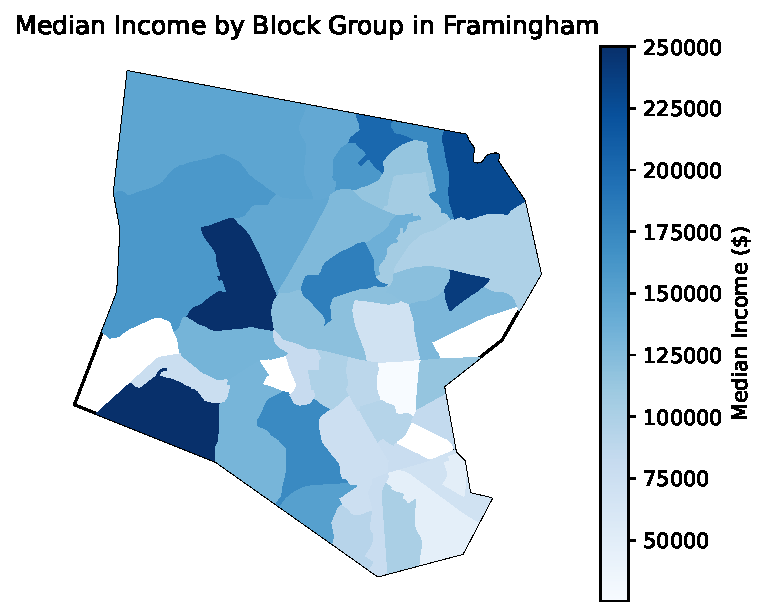
\includegraphics[width=0.99\textwidth, alt={Choropleth map of median income by census block group in Framingham. Darker blue areas indicate higher median income, and lighter areas indicate lower median income.}]{figures/median_income_by_block_group.pdf}
    \end{subfigure}
    \caption{Plots of different socioeconomic factors in Framingham, Massachusetts. Block group boundaries use 2020 U.S. Census geography; income estimates use 2020--2024 \gls{acs} 5-year estimates.}
    \label{fig:geospatial}
\end{figure}

The current assignment therefore reflects both operational routing decisions and upstream policy-driven demand. At present, \gls{fps} uses 51 buses (with a maximum of 86 available) to serve 219 students with disabilities and 4,561 students without disabilities at the identified schools (4,780 riders total, matching \autoref{tab:demographics}).

Additionally, Census-based demographic information was estimated by determining the corresponding block-group for different student addresses, then randomly sampling based on the percentage returned from 2020--2024 \gls{acs} 5-year estimates.

\begin{table}[!htbp]
    \centering{
    \tagpdfsetup{table/header-rows={1}}
    \begin{tabular}{@{}lll@{}}
    \toprule
        Category & Quantity & Avg Dist. to School [mi] \\ \midrule
        All students in \gls{fps} & 8210 & 2.81 \\
        Students currently riding bus & 4780 & 3.55 \\
        Within 1 mile of school & 1085 & 0.62 \\
        Within 2 miles of school & 2412 & 1.35 \\
        Further than 5 miles from school & 531 & 5.36 \\
        Language other than English at home & 4034 & 2.97 \\
        Non-car owning household & 760 & 3.03 \\
        Students with disabilities & 1096 & 2.49 \\ 
        \bottomrule
    \end{tabular}
    }
    \caption{\gls{fps} student demographics and average home-to-school distance by student group, reported in miles. Categories are not mutually exclusive; a student may belong to multiple rows.}
    \label{tab:demographics}
\end{table}

\section{Currently Assigned Students}

The preliminary results indicate that \gls{bra} can improve \gls{fps}'s bus operations while preserving student coverage. Under the tested configuration, the algorithm serves the same 4,780 currently assigned students using 48 buses instead of 51, reducing deployed buses by 3, or approximately 5.9\%. This suggests that the existing network contains meaningful routing inefficiency that can be addressed through algorithmic reassignment and multi-school bus utilization. The core operational advantage of \gls{bra} is that it allows each bus to complete multiple trips across schools, while each trip remains structured around a specific grade and school assignment. For this preliminary test, I use conservative estimates and assume buses travel at an average speed of 30 miles per hour, require 30 seconds for student boarding, 1 minute for boarding students with disabilities, arrive between 10 minutes and 40 minutes before school bell time, and include a required 10-minute dwell time at the school as a buffer.

\begin{table}[!htbp]
    \centering{
    \tagpdfsetup{table/header-rows={1,2}}
    \begin{tabular}{@{}lllllllll@{}}
        \toprule
        Category 
        & \multicolumn{4}{l}{\textbf{Current Routing}} 
        & \multicolumn{4}{l}{\textbf{\acrshort{bra} with Current Students}} \\
        & Mean & StDev & Min & Max 
        & Mean & StDev & Min & Max \\ 
        \midrule
        Currently assigned 
        & 43.08 & 29.00 & 3.05 & 133.38 
        & 30.52 & 14.13 & 1.64 & 58.31 \\
        Non-English at home 
        & 41.24 & 28.16 & 3.91 & 133.38 
        & 31.18 & 13.72 & 1.64 & 58.31 \\
        Non-car owning household 
        & 39.83 & 27.89 & 3.91 & 133.37 
        & 30.66 & 13.28 & 1.64 & 58.23 \\
        Students with disabilities
        & 36.68 & 20.82 & 3.05 & 125.38 
        & 25.35 & 13.33 & 2.14 & 57.86 \\
        \midrule
        Buses used 
        & \multicolumn{4}{l}{51} 
        & \multicolumn{4}{l}{48} \\
        \bottomrule
    \end{tabular}
    }
    \caption{Estimated travel times in minutes for currently assigned riders under current routing versus the \gls{bra} configuration. Does not account for intersection delay, assumes constant bus speed.}
    \label{tab:travel_times}
\end{table}

The benefits are not limited to fleet utilization. Across all tracked student groups, \gls{bra} reduces estimated mean travel times relative to the current routing baseline, as shown in \autoref{tab:travel_times}. For currently assigned bus riders, mean travel time falls from 43.08 minutes to 30.52 minutes, a reduction of approximately 29.2\%, while the maximum observed travel time falls from 133.38 minutes to 58.31 minutes. 

Vulnerable groups also see consistent improvements under the modeling assumptions (\autoref{tab:travel_times}): mean travel time declines from 41.24 to 31.18 minutes for students from households where English is not the primary language, from 39.83 to 30.66 minutes for students from non-car-owning households, and from 36.68 to 25.35 minutes for students with disabilities. Additionally, because mean travel time decreased for non-car-owning households by approximately 23.0\% under \gls{bra}, this suggests that efficiency improvements are not achieved by sacrificing service to transit-dependent households. \autoref{fig:routes_assigned} shows the current and proposed route layouts side-by-side.

\begin{figure}[!htbp]
    \centering
    \begin{subfigure}{0.495\textwidth}
        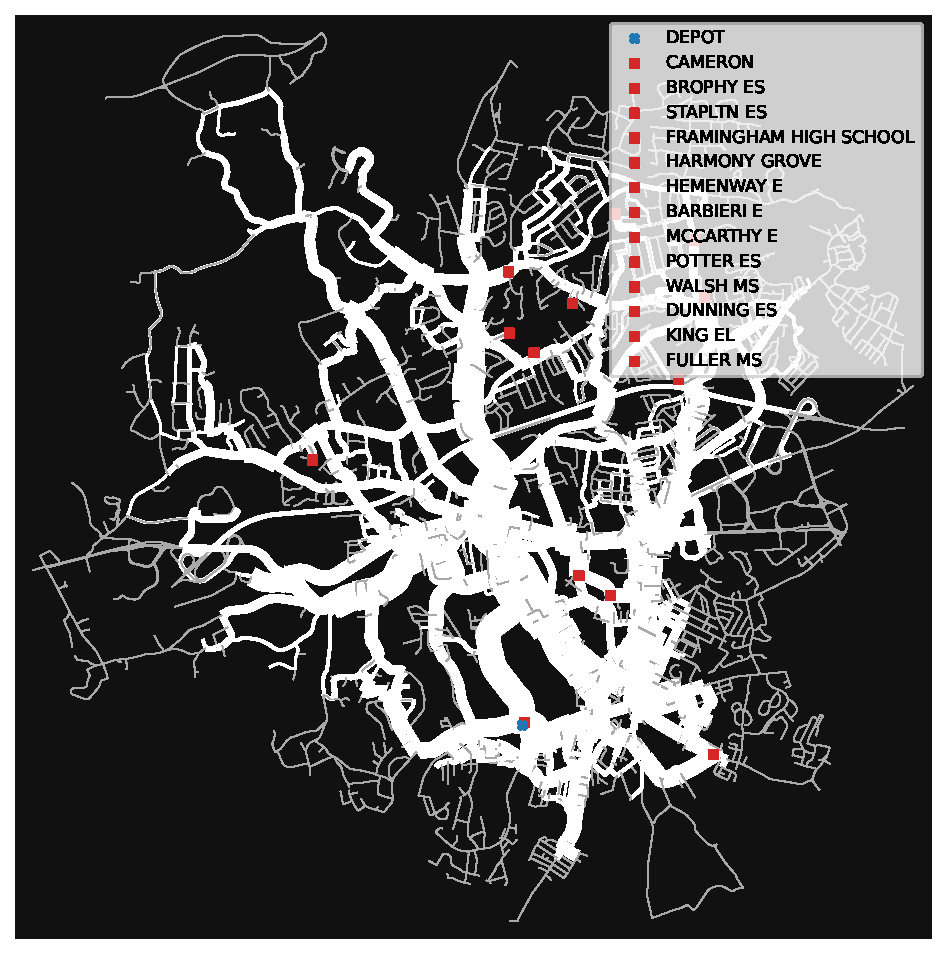
\includegraphics[width=0.99\textwidth, alt={Route-density map of current \glsentrylong{fps} bus routes. White road links indicate roads used by more buses, schools are highlighted in red, and depots are shown in blue.}]{figures/existing_routes.pdf}
        \subcaption{Current routes used by \gls{fps}}
    \end{subfigure}
    \begin{subfigure}{0.495\textwidth}
        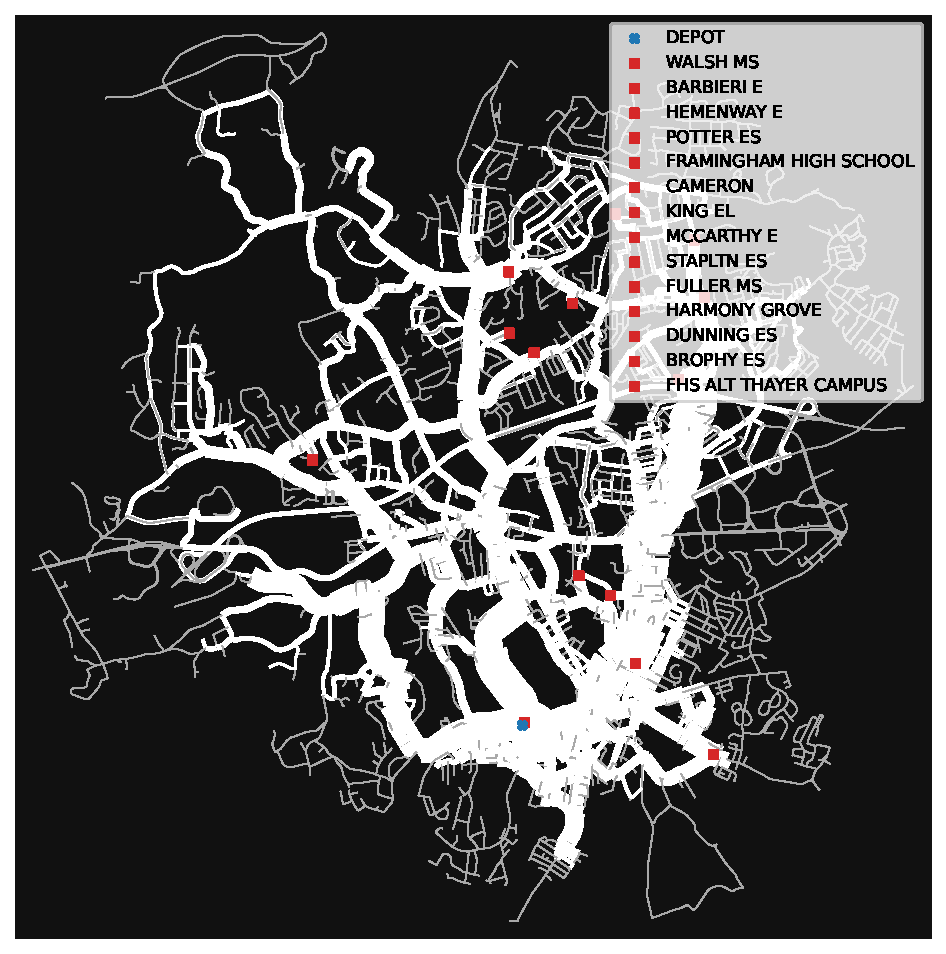
\includegraphics[width=0.99\textwidth, alt={Route-density map of proposed routes generated using \glsentrylong{bra}. White road links indicate roads used by more buses, schools are highlighted in red, and depots are shown in blue}]{figures/bird_assigned_students_routes.pdf}
        \subcaption{Proposed routes generated using \gls{bra}}
    \end{subfigure}
    \caption{Route-density maps of different configurations with currently assigned students, with the width of each road link varying based on how many buses travel along it.}
    \label{fig:routes_assigned}
\end{figure}

\section{All Students}

\gls{fps} is considering moving from an opt-in routing model to an opt-out model, where students are provided school bus service by default. Thus, I applied \gls{bra} with the current fleet constraints and existing stops and found that the current student population living over 1.5 miles\footnote{\gls{fps} is required under Massachusetts law to offer no-cost transportation for students living over 2 miles away. However, as of writing, \gls{fps} also offers bus transportation for students living between 1 and 2 miles away for an associated fee \cite{framinghampublicschoolsRider, framinghamschoolcommittee2022Student}.} from their school can be served using the existing fleet available to \gls{fps}. Conversely, all students in the district with the current bus fleet cannot be fully served with the assumed modeling and operational constraints, as shown in \autoref{tab:travel_times_all}. 

\begin{table}[!htbp]
    \centering{
    \tagpdfsetup{table/header-rows={1,2}}
    \begin{tabular}{@{}lllllllll@{}}
        \toprule
         Category & \multicolumn{4}{l}{\textbf{All Students $\geq$ 1.5 miles away}} & \multicolumn{4}{l}{\textbf{All students}} \\
         & Mean & StDev & Min & Max & Mean & StDev & Min & Max \\ \midrule
         All students 
         & 30.81 & 14.67 & 3.52 & 59.62 
         & 29.67 & 14.95 & 0.73 & 59.76 \\
         Non-English at home 
         & 31.69 & 14.49 & 3.55 & 59.62 
         & 30.77 & 14.47 & 0.73 & 59.43 \\
         Non-car owning household 
         & 32.24 & 14.00 & 4.60 & 59.62 
         & 31.68 & 14.41 & 2.41 & 59.76 \\
         Students with disabilities 
         & 29.93 & 14.37 & 4.55 & 58.26 
         & 30.52 & 15.03 & 2.14 & 59.76
         \\ \midrule 
         Total number of students & \multicolumn{4}{l}{6304} & \multicolumn{4}{l}{8210} \\
         Students unassigned & \multicolumn{4}{l}{0} & \multicolumn{4}{l}{13} \\ 
         Buses used & \multicolumn{4}{l}{62} & \multicolumn{4}{l}{78} \\
         \bottomrule
    \end{tabular}
    }
    \caption{Estimated travel times of students in minutes with different routing configurations with the set of all students. Does not account for intersection delay, assumes constant bus speed.}
    \label{tab:travel_times_all}
\end{table}

\begin{figure}[!htbp]
    \centering
    \begin{subfigure}{0.495\textwidth}
        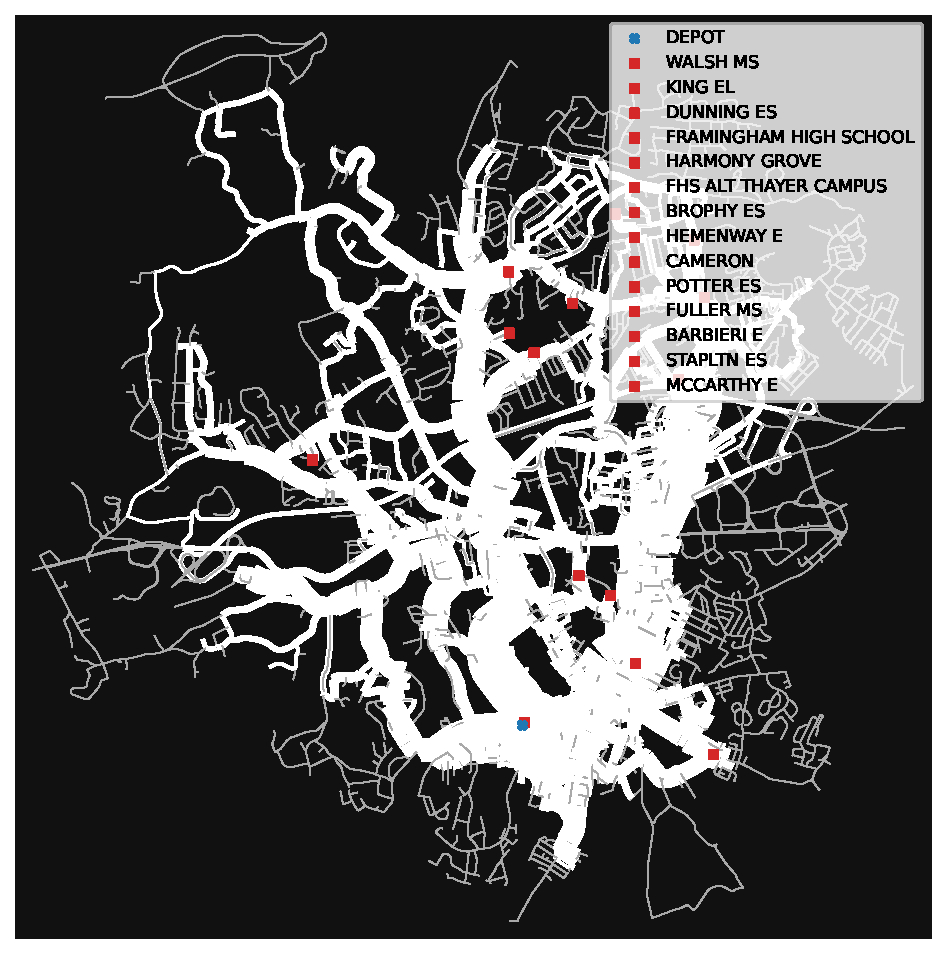
\includegraphics[width=0.99\textwidth, alt={Route-density map of possible routing for students at least 1.5 miles from school. White road links indicate roads used by more buses, with selected route segments highlighted in red.}]{figures/bird_all_students_over_1_5_miles.pdf}
        \subcaption{Possible routing of students $\geq$ 1.5 miles away}
    \end{subfigure}
    \begin{subfigure}{0.495\textwidth}
        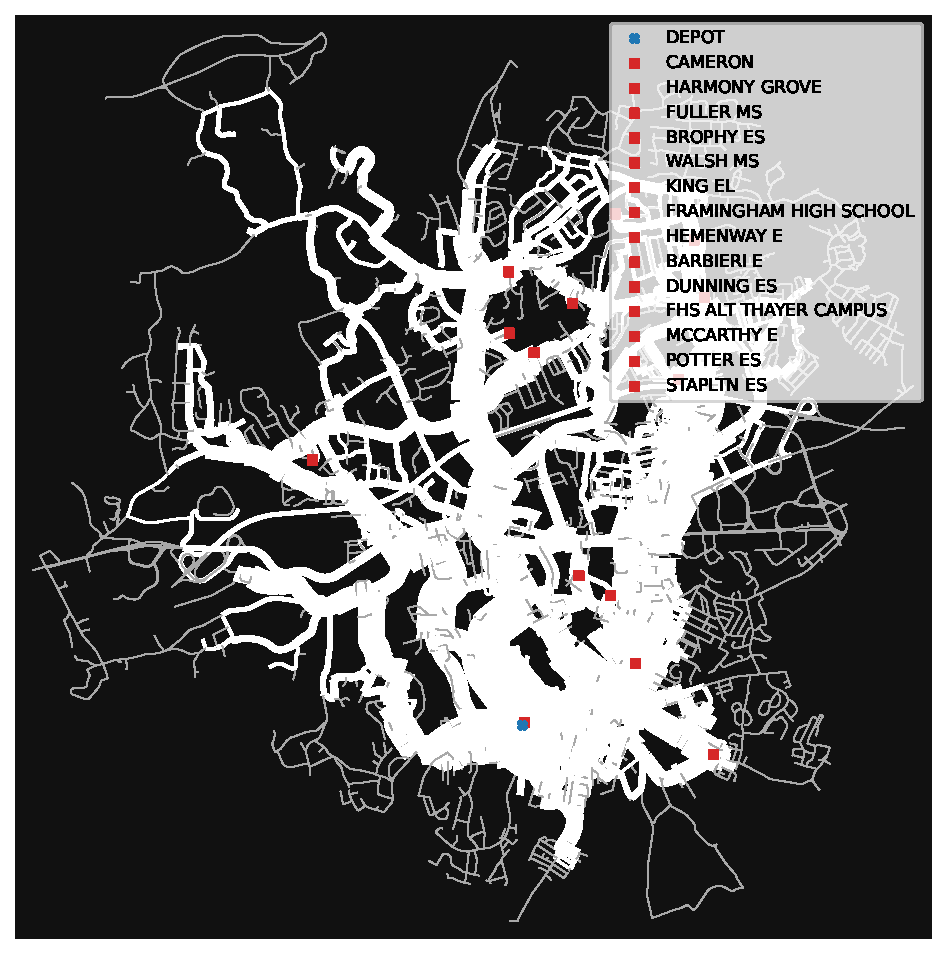
\includegraphics[width=0.99\textwidth, alt={Route-density map of possible routing for all students. White road links indicate roads used by more buses, with selected route segments highlighted in red.}]{figures/bird_all_students.pdf}
        \subcaption{Possible routing of all students}
    \end{subfigure}
    \caption{Route-density maps of different configurations with the full \gls{fps} student dataset, with the width of each road link varying based on how many buses travel along it.}
    \label{fig:routes_all}
\end{figure}

The Pareto fronts in \autoref{fig:pareto} summarize the tradeoffs induced by varying resource limits and objective weights in the \gls{bra} candidate-selection model. Each point represents a feasible routing configuration generated under the same data assumptions but with different priorities over fleet use, coverage, and student travel time. I also analyze the current \gls{fps} routing plan as a baseline design, making it easy to assess whether existing operations are dominated by generated alternatives under the modeled constraints. Because travel times are estimated using simplified speed assumptions rather than calibrated \gls{avl} data, these fronts should be interpreted as relative planning comparisons rather than final operational schedules.

\begin{figure}[!htbp]
    \centering
    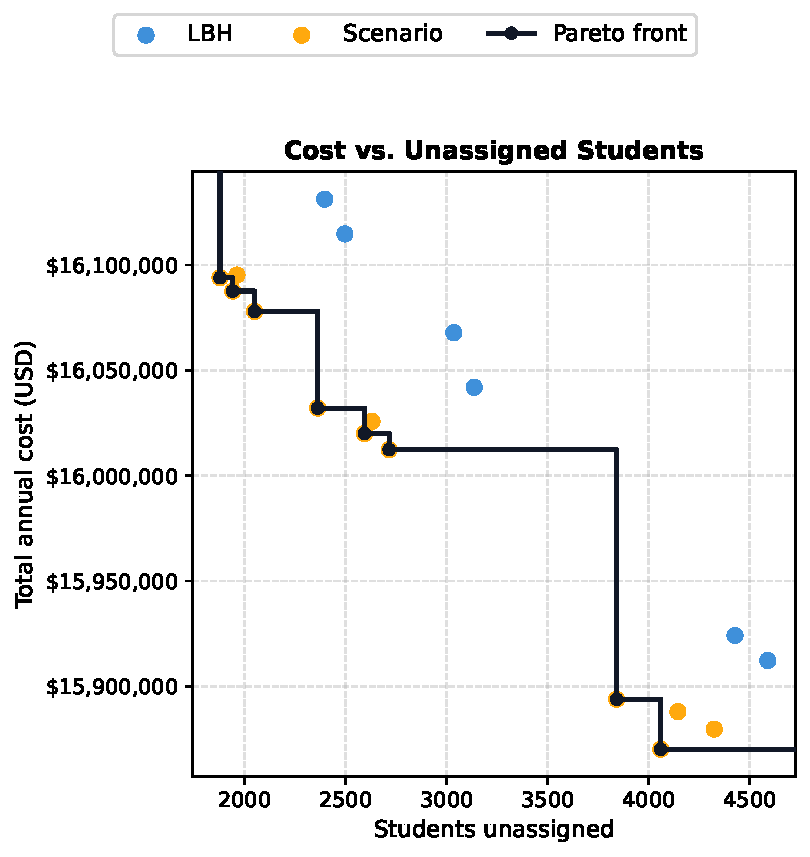
\includegraphics[width=0.4\linewidth, alt={Scatter plot of total annual cost versus students unassigned for \glsentrylong{bird} testing data. \glsentrylong{lbh} and Scenario solutions are plotted to compare how student assignment affects cost.}]{figures/routing_bird_mcdp_pareto_routing_simple_caps_cost_unassigned.pdf}
    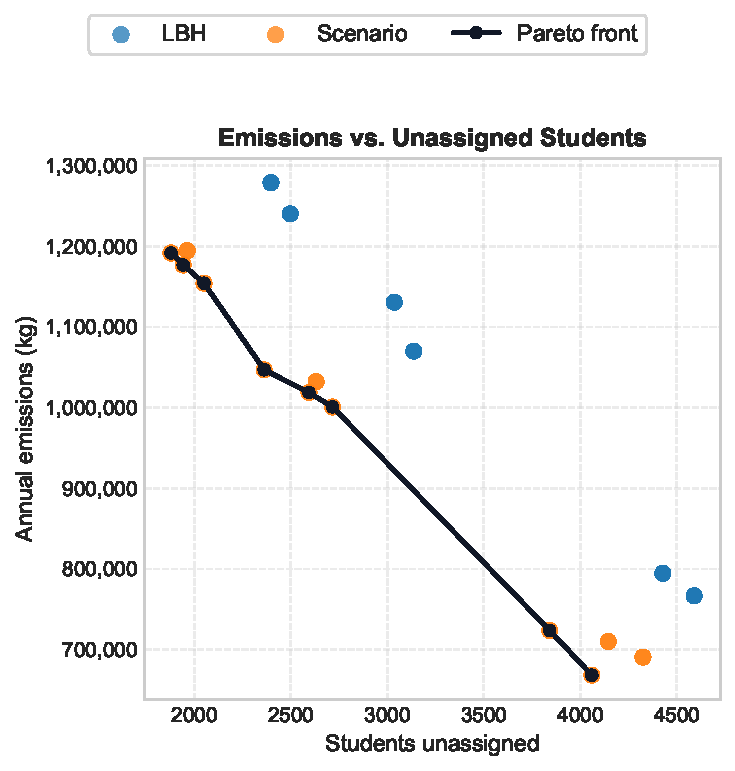
\includegraphics[width=0.4\linewidth, alt={Scatter plot of total annual emissions versus students unassigned for \glsentrylong{bird} testing data. \glsentrylong{lbh} and Scenario solutions are plotted, with the Pareto frontier showing the best emission-coverage tradeoff.}]{figures/routing_bird_mcdp_pareto_routing_simple_caps_emissions_unassigned.pdf}
    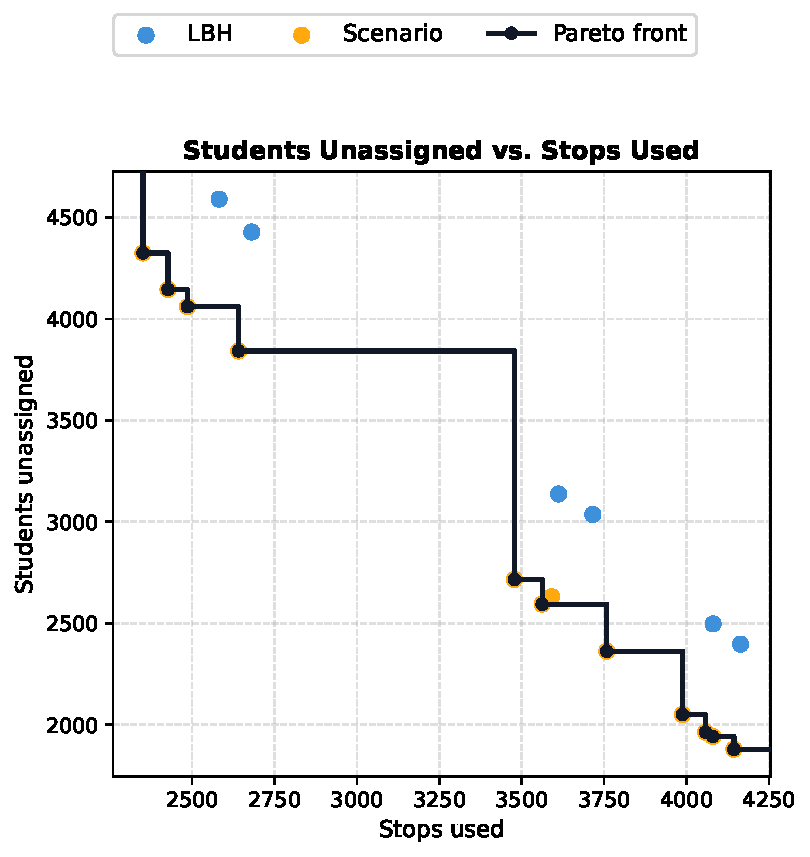
\includegraphics[width=0.4\linewidth, alt={Scatter plot of total students unassigned versus stops used for \glsentrylong{bird} testing data. \glsentrylong{lbh} and Scenario solutions are plotted, with the Pareto frontier showing the best student-stop tradeoff.}]{figures/routing_bird_mcdp_pareto_routing_simple_caps_students_stops.pdf}
    \caption{Pareto fronts for \gls{bra} simplified routing configuration with student data. Each point on these fronts is a valid solution of the co‑design problem with different resource allocations among \gls{mdpi} components (fleet, driver, monitor, fuel, maintenance). The figure makes visible the planning tradeoffs implied by the categorical composition.}
    \label{fig:pareto}
\end{figure}

